\newcommand{\PooledRows}{%
4,096 & 79.80 & 80.29 & +0.61 & 10.3--10.4 \\
32,768 & 79.82 & 80.18 & +0.45 & 82.7--83.4 \\
131,072 & 79.27 & 79.09 & -0.22 & 331.1--334.0 \\
}

\begin{abstract}
How many bits of a prefix must an inference engine carry across a restart to preserve its future answers? For softmax attention on the unit sphere we determine the leading bit cost of a single checkpoint, with known prefix length, fixed dimension and temperature, and uniform error over all continuations. The normalization mass costs as much, to leading order, as one additional value coordinate. A pair of suffixes recovers that mass. Spherical harmonic decay determines how finely each observable coefficient must be stored. We relate this result to the minimum continuous streaming dimension and examine two storage contracts in Qwen3.5-0.8B. An exact-key, bounded-value cache saves 21.1--21.7\% of reserved KV storage; pooled decoding throughput changes by $-0.22$ to $+0.61$\% across three context lengths. For bitwise restart of recurrent matrices, an exact reference selector saves 106,994 bytes across 42.5 million FP32 words. A format lower bound explains the remaining gap to bit shuffling and Zstandard. A one-byte selector between the two formats saves a further 1,357,991 bytes over the smaller fixed format. The three results locate the cost in the information that future reads expose, the numerical error a codec permits, and the bytes its layout actually spends.
\end{abstract}

\noindent\textbf{Code availability.} \codesentence

\section{What must cross a restart?}
Two attention heads can produce zero at every query on two different histories. If the historical values were all zero, those reads say nothing about how much attention mass the keys accumulated. Append a token with value one. The two outputs can now differ, because the new token competes with different masses. An inference checkpoint must preserve enough of the past to answer that next question as well.

In a hybrid decoder, the same restart can ask for two different objects. An attention cache may tolerate perturbations in values if the error of a projected read is small. A recurrent matrix may have to arrive bit for bit so the native update can continue from exactly the saved state. An error tolerance has units; a checkpoint also has a reader, an update rule and a physical layout. We use these distinctions to compare the following results.

\begin{center}
\small\begin{tabular}{@{}p{.25\linewidth}p{.35\linewidth}p{.31\linewidth}@{}}\toprule
Contract & What a future operation can inspect & Quantity determined here\\\midrule
Uniform spherical attention & Arbitrary queries and common suffixes; fixed $d,p,\beta$ & Sharp asymptotics in real coordinates and in bits for one checkpoint\\
Exact keys, bounded values & A shared-value read at fixed keys, queries and gates & Exact projected error radius; measured bytes and decode times\\
Bitwise recurrent restart & Every word restored before a deterministic update & Exact reference optimum and byte floor within a specified format\\\bottomrule
\end{tabular}
\end{center}

The bridge is the set of histories a decoder can safely represent by one message. For ideal attention we construct that set using a future-read distance. For the KV codec we bound the diameter of a value-error box in projected output coordinates. For exact restart, two different native word arrays cannot share a decodable representation. The engineering cases expose constraints that the information bound deliberately leaves free, including arithmetic precision, record framing and the cost of rebuilding a cache.

\section{Sharp memory bounds for resumable softmax attention}\label{sec:setup}
A token carries a unit key $k\in\mathbb S^{d-1}$ and a value $v$ in the Euclidean unit ball of $\mathbb R^p$. For a unit query $q$, fixed $\beta>0$ and a nonempty prefix, define
\[
 Z(q)=\sum_i e^{\beta q^\top k_i},\qquad N(q)=\sum_i e^{\beta q^\top k_i}v_i,\qquad y(q)=N(q)/Z(q).
\]
Keys, values, queries and suffixes may be chosen independently of a language model. The source of each lower bound is the ability to ask new questions of an old prefix. In two one-token tests, append the same key of weight $b>0$ with value $0$ or a unit vector $e$. The output difference $be/(Z+b)$ determines $Z$ and then $N$. Two finite prefixes are interchangeable under every common continuation exactly when their key multiplicities and their value sums at each distinct key agree. The proof in Appendix~\ref{sec:exact} identifies finite atomic measures from their exponential transforms.

\paragraph{Two budgets.}
In a streaming head all access to the past goes through $r$ persistent real coordinates. Every fixed-length input history maps continuously to its state; the time index is free. Write $r_*(\eps)$ for the least dimension achieving Euclidean error at most $\eps$ on every finite stream. Alternatively, cut a length-$n$ history once. The encoder sends a fixed-width bit string; the decoder knows $n$ and receives the exact suffix. Working storage on either side of the cut is unrestricted. Minimize bits at each $n$, then take the supremum over $n$, to define $\Bchk(\eps)$. Both budgets have free-key variants in which the exact prefix key history is available and only value-dependent storage is charged. The streaming free-key state must be continuous at fixed keys. The one-shot encoder may quantize discontinuously.

\begin{theorem}[Cost of the normalization mass]\label{th:unified}
Fix $d\ge2$, $p\ge1$, $\beta>0$. Let $T=\log(1/\eps)$ and $m_T=T/\log T$. Write $c=p+1$ for joint storage or $c=p$ when keys are free. In the corresponding models, as $\eps\downarrow0$,
\begin{equation}
 r(\eps)\sim \frac{2c}{(d-1)!}\,m_T^{\,d-1},
 \qquad
 B(\eps)\sim \frac{2c}{d!\log 2}\,T m_T^{\,d-1}.
 \label{eq:both}
\end{equation}
These constants also hold when an input rotation acts on all previous keys before insertion and a fixed continuous orthogonal representation acts on their values.
\end{theorem}

For scalar values on the circle, the need to represent the key history's effect doubles both leading costs. At general $p$ their joint-to-free ratio tends to $(p+1)/p$. The bit cost is smaller by a factor tending to $d$ than assigning $\log_2(1/\eps)$ bits to every coordinate in the optimal-order streaming dimension with its sharp constant. The two optimal objects have different admissible computations. The theorem evaluates each in its own model.

\begin{figure}[t]\centering
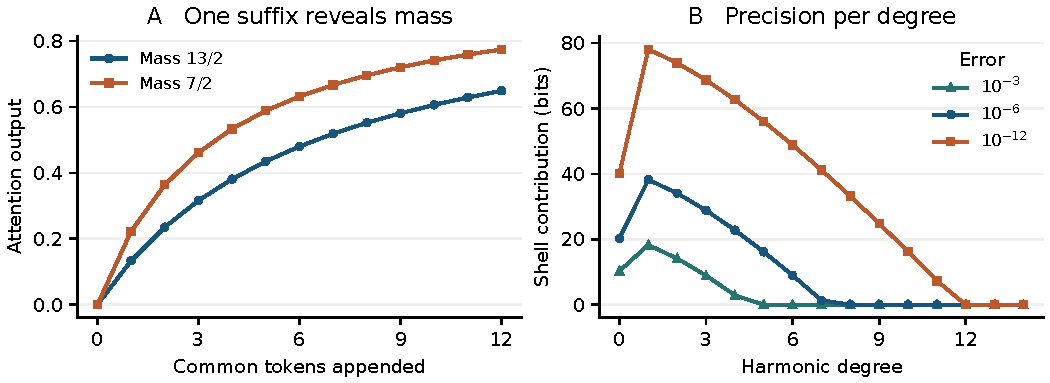
\includegraphics[width=.98\linewidth]{figures/checkpoint.pdf}
\caption{Left: two zero-valued length-four prefixes give different answers after adding the same value-one tokens. At the first append, the gap is $4/45$. Right: the spectral sum underlying the bit proof on the circle at $\beta=1$. Each point is $h_\ell[\log_2(\lambda_\ell/\eps)]_+$ for one scalar channel, before the lower-order covering terms. The vertical scale gives contributions to that sum.}\label{fig:witness}
\end{figure}

\paragraph{Why the bit constant has a factorial $d!$.}
Let $h_\ell$ count the degree-$\ell$ spherical harmonics. There are about $2m^{d-1}/(d-1)!$ modes through degree $m$. Their exponential-kernel eigenvalues satisfy $\log\lambda_\ell=-\ell\log\ell+O_{d,\beta}(\ell+1)$ for $\ell\ge1$. For the upper bound, encode the normalized historical mass and numerator in harmonics. High degrees have small amplitude even when the history is arbitrarily long. Quantizing each coefficient to an absolute tolerance determined by $\eps$ gives a bit cost governed by
\[
  \frac{c}{\log 2}\sum_{\ell} h_\ell[T+\log\lambda_\ell]_+ .
\]
For the converse, length-matched positive and negative suffixes distinguish mass and numerator with stable constants. Independent bounded perturbations to the key density and to each value density then produce a full harmonic ellipsoid of observable prefixes. A packing of the ellipsoid can be realized by ordinary tokens of one common length, even with identical keys in the free-key experiment. Integrating the fraction $1-\ell/m_T$ of significant precision across retained modes gives $1/d$. Appendix~\ref{app:entropy} proves the covering and packing bounds with the same leading constant.

\paragraph{Why the streaming dimension has a different proof.}
Positive polynomial approximations to the kernel yield a recurrent moment matrix. Degree $m$ suffices when the upper Poisson tail at mean $2\beta$ is sufficiently small. For the lower bound, weighted spherical designs put independent mass and value signals in low harmonics. Realizing those weights continuously by fixed-length ordinary token streams makes Borsuk--Ulam applicable to any continuous encoder. Its colliding antipodes admit a separating common suffix. Appendix~\ref{sec:finite} gives the finite inequalities, construction and limiting argument. For instance, with $d=3$, $p=2$, $\beta=1$ and $\eps=10^{-6}$ they certify $74\le r_*(\eps)\le588$. The exact finite optimum is open even in this example.

\section{What keeping exact keys buys in a finite cache}\label{sec:kv}
The free-key theorem asks what remains chargeable once keys are known. A real codec that chooses exact keys must pay to store them. It does gain a precise local certificate: at common queries, keys, masks and gates, the attention probabilities are identical in exact arithmetic. Only value residuals enter the ideal projected difference. Let $a_{hi}$ be the probability at visible position $i$ for query head $h$, $g(h)$ its KV group, $s_{hc}$ a fixed channel gate, and $W$ the output projection. If $|e_{gic}|\le\eta_{gic}$, the sharp worst-case projected $\ell_\infty$ error is
\begin{equation}
 \max_j\sum_{g,i,c}\eta_{gic}\left|\sum_{h:g(h)=g} W_{j,hc}s_{hc} a_{hi}\right| .
 \label{eq:localbody}
\end{equation}
Heads in one group share an error variable. One can attain the radius by choosing its sign from a maximizing combined row. Two heads with equal probabilities, gates one and opposing projections cancel exactly. If $|s_{hc}|\le1$ and every tolerance is at most $\eta$, the radius is at most $\eta\|W\|_{\infty\to\infty}$. Appendix~\ref{app:math} gives the proof, an exact characterization of invisible residuals with affine scores and the additional stability assumptions required to protect a greedy token.

\paragraph{Deployed representation.}
In Qwen3.5-0.8B, 18 recurrent layers and six full-attention layers share the decoding loop \cite{qwen,gdn}. The tested attention reader stores a 256-coordinate BF16 key row in 384 bytes when its exponent range fits, otherwise 512. A value row uses 352 bytes when reconstruction passes its absolute budget and 512 otherwise. The implementation chooses a tolerance just below $1/(128\|W\|_{\infty\to\infty})$ in each layer. Two four-byte headers bring the minimum K/V pair to 744 bytes; a raw key adds 128 and a raw value adds 160. In a packed prefix the encoder pays for the selected modes. For each future token the allocator reserves full-width slots over six layers and two groups: 12,384 bytes, compared with 12,288 in dense BF16. The output error $1/128$ concerns the ideal projection at fixed inputs. Kernel rounding and changes in hidden state have separate effects.

\begin{table}[t]\centering\small
\caption{BF16 Qwen3.5-0.8B on one RTX PRO 6000 Blackwell. For each prefix length, each backend generated 64 tokens in four runs on each of two books. Rates pool tokens divided by elapsed seconds. The final column spans the two observed KV reservations.}\label{tab:rates}
\begin{tabular}{rrrrr}\toprule Prefix (tokens)&Dense (tok/s)&Compact (tok/s)&Change (\%)&Saved (MiB)\\\midrule
\PooledRows\bottomrule\end{tabular}
\end{table}

\paragraph{A whole-model measurement.}
The baseline is dense FlashInfer \cite{flashinfer}. Both paths share projections, recurrent updates and greedy selection. Batch size is one. We take three nested prefixes from each of \emph{Emma} and \emph{Moby-Dick} \cite{nltk}. A warm-up precedes four pairs with alternating order. Timed steps include appending a new K/V record and returning its token ID to Python. All 384 positions in the six distinct continuations match. Pooled throughput varies by less than one percent in either direction (Table~\ref{tab:rates}); the 24 individual timing pairs appear in Appendix~\ref{app:record}. At 131,072 tokens the cache saves 331.1--334.0 MiB. Converting the prefix takes 14.93--15.94 seconds once, which raises the reconstructed single-request total from about 10 seconds to 24.94--25.93 (Figure~\ref{fig:budget}). The reported storage excludes weights, recurrent states and workspace. The six continuations quantify observed agreement; subsequent queries and gates in an autoregressive run need not coincide.

\begin{figure}[t]\centering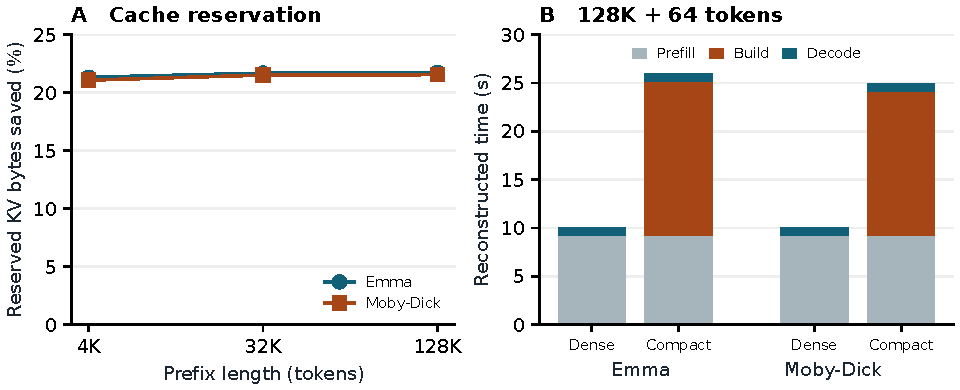
\includegraphics[width=.95\linewidth]{figures/budget.pdf}
\caption{Prefix packing saves KV capacity across the six conditions. At 128K the right panel separates common prefill, cache construction and 64 warm generation steps. Host conversion and kernel preflight are included in the measured compact build.}\label{fig:budget}
\end{figure}

\section{When every recurrent word must survive}\label{sec:word}
A bitwise restart requires the inverse codec to return exactly the original words. If the remaining machine state, arithmetic and inputs are identical, determinism then preserves all later native transitions by induction. Small approximation error alone gives no compression guarantee for this contract. For example, set $X_{ij}=1+2^{-23}d_{ij}$ with $0\le d_{ij}<2^s$, $s\le23$. These positive FP32 matrices lie within relative squared Frobenius error $((2^s-1)2^{-23})^2$ of the all-ones rank-one matrix. They still contain $s$ freely chosen bits per entry (Appendix~\ref{app:words}).

\paragraph{A lower bound that can guide an encoder.}
Consider a row of 128 binary32 words. Within sixteen groups of eight, encode the 31-bit magnitude $a_i$ relative to an integer reference $t$, using a common width per group and a separate sign stream. For $\mathrm{zz}(z)=2z$ for $z\ge0$ and $-2z-1$ otherwise, the width is the bit length of the largest ZigZag residual. If group extrema are $l_j,h_j$, width at most $w\ge1$ is equivalent to
\[
  h_j-2^{w-1}+1\ \le t\le\ l_j+2^{w-1}.
\]
Width zero gives a singleton for a constant group. Each width threshold therefore contributes a known saving over an interval. Sweeping their weighted endpoints yields a global optimum, including byte rounding and ties. With $s$ sign-exception masks, let $R_0,R_*$ be baseline and optimal residual record lengths, and $A$ the cheapest alternative (raw, exponent or zero). The complete record gains exactly $[\min(R_0-R_*,A-R_*)]_+$. Grant each group a distinct free reference and the fixed-header floor becomes
\[
 \min\!\left(A,\,17+4s+\sum_j\left\lceil\log_2(1+h_j-l_j)\right\rceil\right).
\]
Both conclusions apply to an explicit layout. Changing the transform or entropy-coding across rows can cross the floor. Appendix~\ref{app:one} gives the optimization algorithm, a checkable certificate, and an extension to multiple stored references.

\begin{table}[t]\centering\small
\caption{Exact FP32 reconstruction on 2,592 archived heads. Lengths include implemented framing except for the native array. The floor grants free group references with the residual header fixed.}\label{tab:bytes}
\begin{tabular}{@{}lr@{}}\toprule Representation & Total bytes\\\midrule
Dense native words &169,869,312\\
Row modes, midpoint reference &149,047,714\\
Row modes, optimal reference &148,940,720\\
Fixed-header lower bound with free group references &148,335,505\\
Bit shuffle and Zstandard, whole-head frames &142,093,897\\\bottomrule
\end{tabular}
\end{table}

\paragraph{How much of the optimum survives mode selection?}
Three teacher-forced Q4\_0 traces supply all 18 recurrent layers and 16 heads at tokens 1, 428 and 460. This is a separate offline experiment from the BF16 attention run. We serialize and decode every $128\times128$ FP32 head and compare the words. Exact selection saves 2,045,888 candidate bytes, of which 106,994 (5.23\%) survive competition with the other row modes. At aggregate level, even free group references leave 6,241,608 bytes above bit shuffle plus Zstandard (Table~\ref{tab:bytes}). The ordering reverses at each of the two later checkpoints: the optimized local layout is about 0.48--0.59 MB smaller there. The first checkpoint and its equal weight in the census explain the aggregate. A whole-head compressor and a sequential row decoder also expose different access granularities. These figures describe archived words and the specified layouts; they do not measure online recurrent decoding speed.

\paragraph{An implementable consequence of the floor.}
The two frame formats win on different heads. Encode each head both ways, choose the shorter complete frame, and write one selector byte before its existing four-byte length field. An independent pass parses the resulting stream, decodes exactly one selected frame per head, and compares all recovered words against the original. The 2,592-head file occupies \textbf{140,735,906 bytes}, including every selector. It chooses the local format 1,522 times and bit shuffle 1,070 times, improving on always using bit shuffle by 1,357,991 bytes (0.96\%). This gain comes from a change of representation at head granularity. Encoding both candidates incurs extra work. We did not time the selector or test it in a live model. Appendix~\ref{app:mixed} reports the checkpoint breakdown.

\section{Relation to prior work and limits}\label{sec:scope}
Kernel-feature attention stores an unnormalized value sum and a normalizer \cite{kath,schlag}. Streaming attention bounds based on communication reductions, discrepancy, polynomial approximations and partitioning study resource models with explicit bit or stream constraints \cite{haris,balance,chen}. Query-distribution risk supplies another objective \cite{risk}. Our continuous dimension result concerns deterministic uniform accuracy in fixed dimension. The bit theorem charges one message and grants exact suffix storage. It cannot be applied as a constant-memory implementation of repeated finite-precision updates. Work on isotropic kernels already relates spherical spectra to covering numbers \cite{entropy}, while nonlinear widths characterize approximation by continuous parameters \cite{devore}. The extra steps here are to recover both profiles from common continuations and realize a matching packing by valid prefixes.

KIVI quantizes keys and values on different axes \cite{kivi}; bounded-error quantized attention propagates score and value errors \cite{calver}; weighted value projection accounts for attention priorities \cite{salfati}. Equation~\eqref{eq:localbody} takes the support function after grouping the shared variables. Integer frame-of-reference coding, floating-point layouts and bit shuffling provide the coding context for the recurrent experiment \cite{lemire,alp,shuffle}. Its format floor can distinguish an exhausted reference search from a potentially better layout.

The theoretical sphere, arbitrary suffix values, exact arithmetic and asymptotic accuracy do not describe the measured model's reachable states. The empirical evidence covers one GPU session, two books and 64-token continuations for attention, and three traces with three checkpoint positions for recurrent words. No run used both codecs together. Adding their byte percentages would mix distinct denominators, precisions and workloads. Joint deployment would require measuring total peak device memory, prefix reuse, recurrent serialization and the resulting token sequence in one execution. For the existing runs the defensible conclusion is narrower: keeping a normalizer has a quantifiable information price, while a concrete decoder's storage and latency depend on where and how it pays that price.

\paragraph{Reproduction.}
The CPU notebook regenerates the figures from harmonic calculations, one archived GPU trace and a per-head census. It checks exact arithmetic witnesses and re-encodes a portable raw-word subset. The appendix gives the full protocols, resource boundaries and AI-assistance disclosure. The anonymous copy includes the conference checklist.

